\section{Theorie}
\label{sec:theorie}
\subsection{Totzeit}
Die Totzeit ist diejenige Zeit die verstreichen muss, bis wieder neue Zählungen
aufgenommen werden können.
Sie kommt daher zustande, dass nach der Ionisation die positiven Ionen, welche
deutlich schwerer sind als die Elektronen, sich wesentlich länger im Bereich
zwischen Anode und Kathode aufhalten. Sie bauen ein radialsymmetrisches Feld auf,
welches das elektrische Feld abschirmt, sodass keine Stoßionisation mehr
auftritt und keine Impulse aufgezeichnet werden können. Wenn die Kationen zur
Kathode wandern, wird die Feldstärke allmählich größer und es können wieder
Impulse detektiert werden.

\subsection{Nachentladungen}
Nachentladungen treten dann auf, wenn Ionen, die an der Zählrohrhülle
neutralisiert werden, dort Elektronen herauslösen. So können durch ein
einziges Teilchen mehrere Impulse aufgezeichnet werden, welche also Zählungen
vortäuschen. Dieser Effekt wird minimiert, wenn das Edelgas im Inneren des
Rohres mit Alkoholdampf vermischt wird. Die Elektronen ionisieren so den
Alkohol. Dieser wird dann an der Anode neutralisiert, löst aber keinen Impuls
aus. Die Energie wird in die Schwingung dieser vielatomigen Moleküle gesteckt.

\subsection{Charakeristik des Zählrohrs}
Bei der Charakteristik eines Zählrohrs wird die Anzahl der registrierten
Teilchen gegen die angelegte Spannung U aufgetragen.
Die so entstehende Kurve, vgl Abbildung \ref{fig:char},
weist einen Bereich mit ungefähr konstanter Steigung
auf, welcher Plateau genannt wird. Die Plateaulänge ist dabei ein Maß für den
Arbeitsbereich des Zählrohrs. Umso geringer die Steigung des Plateaus ist, desto
besser arbeitet das Zählrohr. Aufgrund von Nachentladungen kann die Steigung
aber niemals Null werden.

\begin{figure}
  \centering
  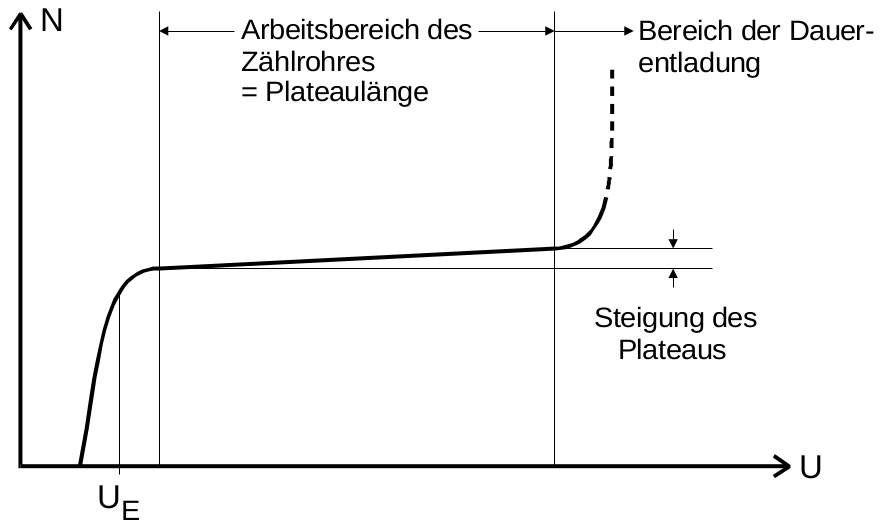
\includegraphics[width=10cm]{content/charakteristik.png}
  \caption{Schematische Skizze der Charakteristik eines Zählrohres. \cite{Anleitung}}
  \label{fig:char}
\end{figure}

Zählrohre funktionieren bei $α$ -und $β$-Strahlung sehr gut, da die Strahlungen
ein hohes Ionisationsvermögen aufweisen.

\subsection{Zwei Quellen Methode}
\label{sec:zweiquellen}
Die Totzeit führt dazu, dass die Tatsächliche Menge an Zählungen $N_r$ kleiner
ist als die Menge der pro Zeiteinheit absorbierten Teilchen
\begin{align}
    N_w &= \frac{\text{Impulse}}{\text{Messzeit}}\:.
    \intertext{Bei der Zwei-Quellen-Methode werden für zwei Strahlungsquellen
    die einzelnen Intensitäten $N_1, N_2$,
    sowie die kombinierte Intensität $N_{1,2}$ gemessen.
    Es sollte}
    N_{1,2} &= N_1 + N_2
    \intertext{gelten, es ist aber}
    N_{1+2} &< N_1 + N_2\:.
    \intertext{Die wahre Teilchenzahl einer Quelle ist}
    N_\text{1,w} &= \frac{N_1}{1-T_\text{t}\cdot N_1}
    \intertext{mit der Totzeit $T_\text{t}$
    Mit der Herleitung aus \cite{Anleitung} folgt die Näherung}
    T &\approx \frac{N_1 + N_2 - N_{1+2}}{2 N_1 N_2}\:.
    \label{eqn:zweiquellen}
\end{align}

\subsection{Messung mittels freigesetzter Ladungsmenge}
Mit einem Amperemeter kann der Zählrohrstrom $\bar{I}$ gemessen werden.
Da ein Strom gerade Ladung pro Zeiteinheit ist,
\begin{equation}
    \bar{\symbf{I}} = \frac{\increment Q}{\increment t} Z
    \label{eqn:ladung}
\end{equation}
kann dadurch die einfallende Ladung $\increment Q$ in Äbhängigkeit der
Teilchenzahl bestimmt werden.
